%!TEX root = ../main.tex
\section{Background}
\label{sec:background}
In this section, we detail the foundational concepts behind our approach.
We introduce the basic networking models in Section~\ref{netw_model}.
Then, we discuss the concept of SRTs in detail in Section~\ref{subsec::srt} as well as the common parent selection scheme in Section~\ref{subsec::parent}. 
Finally, we introduce the actor networking model that Rime employs in Section~\ref{subsec::actor}.

\subsection{Networking Model} 
\label{netw_model}
Edge deployments combine two main networking models: \textit{1) flood-like}~\cite{levis2008emergence} and \textit{2) index-based}~\cite{pietzuch2006network} networks. Flood-like networks are highly distributed and peer-to-peer (P2P) or P2P-like and assume that nodes are capable of moving. In contrast, index-based networks use meta-information about the physical topology for making routing decisions on the application level.%\steffen{it is not totally comprehensible what you want to say here}

Nodes in a flood-like network broadcast (flood) messages across the network in order to propagate information and processing. To this end, flood-like networks usually employ a multi-hop design for messages~\cite{aggarwal2013managing}. 
As a result, nodes can not rely on the topology to be the same during the entire broadcast duration.
One example of a flood-like network is a WSN, where processing and communication are fully decentralized.
Sensor nodes gather and process data in-situ to reduce transmission costs and later forward results to a sink
through multi-hop communication.
% \steffen{,maybe say one more sentence how this is applied in wsn eg. root node etc}

Index-based approaches utilize centralized indexes for book-keeping of metadata, which supports decision making. 
Applications can access the index and make routing decisions timely, as the index is in main memory. Depending on the application, the index can be centralized or decentralized~\cite{muhl2006distributed}. 
The nodes can utilize the index for making any decision and can assume that the topology is reliable. 
An example of such an application is an \textit{overlay} network of data-centers, where a data structure keeps track of link-qualities between nodes and later categorizes them based on that attribute. 
An external application (e.g.: a stream processor) can later utilize that meta-information for performing operator placement.
%
\begin{figure}[t]
  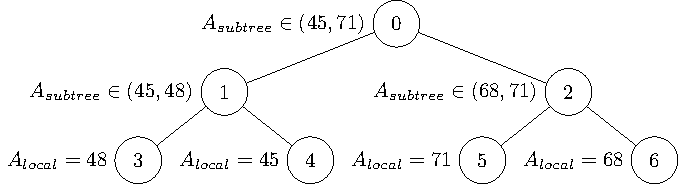
\includegraphics[width=0.46\textwidth]{img/vliot-basic-srt/vliot-basic-srt.pdf}
  \caption{Exemplary topology with an SRT over Attribute $A$. Parents only know the attribute range within their subtree.}
  \label{fig:basic-srt}
\end{figure}
%

\subsection{Semantic Routing Trees} 
\label{subsec::srt}
% 
TinyDB~\cite{madden2005tinydb} introduces the concept of \textit{SRTs} to bridge the gap between a flood-like and index-based approach.
% 
SRTs are data structures that stem from work on WSNs and they store information for each node, e.g., the value range that the node produces. In an SRT, nodes fall into the categories of parents, children, or both. A parent keeps track of its children and their attribute values. The attribute values determine what data is produced by the node, e.g.: CO2 emission readings or temperature data between 2 and 8 degree centigrade. In contrast, a child node produces values from sensed phenomena but might also acts as an intermediate parent, for multi-hop communication. The main task of a parent is to decide if its children need to participate in a query and if required, it will route any necessary information to them.

In Figure~\ref{fig:basic-srt}, an SRT acts as a 
distributed index over an attribute \textit{A}. \textit{$N_{0}$} is the root of the tree with
an index over \textit{A} that contains values in range \textit{$(45, 71)$}.
\textit{$N_{0}$} is the parent of \textit{$N_{1}$} and \textit{$N_{2}$},
with ranges of \textit{$(45, 48)$} and \textit{$(68, 71)$}. 
The range of \textit{$N_{1}$} stems from the values of \textit{$N_{3}$} ($48$) and \textit{$N_{4}$} ($45$).
If a query requires values in the range \textit{$(45, 47)$}, then
only the subtree of \textit{$N_{1}$} replies to the query and the other whole
subtree of \textit{$N_{2}$} is ignored.
This process allows SRTs to avoid unnecessary communication because  
a parent node knows the range of all values of its children. The parent node is also responsible for disseminating only relevant queries to its children. 
The main implication is that the choice of a parent strongly affects future maintenance costs and query latency~\cite{madden2005tinydb}; thus, parent selection is an important performance factor. 
% 

\subsection{Parent Selection} 
\label{subsec::parent}
% 
% In an SRT, nodes fall into the categories of parents, children, or both. 
% A parent keeps track of its children and their attribute values. The attribute value is the values that the nodes produce, e.g.: CO2 emmission readings. \steffen{this is too late as it was already used before}
% In contrast, a child node produces values from sensed phenomena but might also acts as an intermediate parent, for multi-hop communication. A parent decides if its children need to participate in a query and if required, it will route any necessary information to them.
% \steffen{I would merge this with the one before}

When a new node enters the network, choosing a parent from a set of candidates or choosing to become a parent impacts query performance as well as future maintenance overhead. 
Ideally, a parent has children that produce values with small variation, such that the range of attribute \textit{A} is small, e.g., temperature values only differ by several degree.
%\steffen{I think you mean domain}
A small attribute range affects the number of children that a parent will adopt as well as the number of topology updates. In the presence of multiple candidate children nodes, parents prefer children that produce \textit{similar} values to their attribute range.
% \steffen{I think they in theory accept all but they should only accept similar ones}
% Tree organization impacts immediately the number of updates over the tree.

In order to stay updated with minimal performance impact, the SRT uses a \textit{neighbor tracking policy}.
This policy is responsible for parent assignment and determines how to propagate updates in the network. The original multi-hop, broadcast-based SRT design does not consider 
information exchange across nodes that are multiple hops away from each other. This communication limitation stems from the energy preserving design of WSNs, as antenna communication is the main culprit of energy expenditure.
Thus, parents in WSNs only have partial knowledge of the network, which exacerbates the effects of a bad assignment and increases communication overhead for SRT updates. In the IoT, we can augment the tracking policy with different networking schemes in order to propagate SRT updates further than just the antenna range of a node.
% \steffen{here too, maybe use my volcano example to make it clear what you mean here}

% neighbor tracking policy helps decide new nodes and further updates
% Therefore the parent selection strongly affects the overall quality
% of a tree, thus also query dissemination and number of messages. 

% Existing work on in-application routing using SRTs focuses on 
% WSNs~\cite{madden2005tinydb}. The authors consider mobility
% as one limiting factor for maintaining SRTs, since choosing a parent
% node in the tree after a failure affects the workload of maintenance.
% Parents are not able to exchange meta-information about their trees
% and can make decision only with local knowledge.

% Recent work on network-aware SPEs for the Fog era focuses on \textit{a-priori} allocation of alternative data paths~\cite{okeeffe2018frontier}. 
% The paths are used to maximize parallelization as well as enable timely failure 
% recovery. On the other hand, an \textit{a-priori} approach does not consider 
% data paths that form \textit{while} the system is online, thus leaving no 
% room for exploitation of ad-hoc alternatives.

% \textbf{Actor Networking.} \steffen{say a more general sentence about actors, e.g. that they represent components that interact with each other from wikipedia: hat treats actor as the universal primitive of concurrent computation. In response to a message it receives, an actor can: make local decisions, create more actors, send more messages, and determine how to respond to the next message received.
% }

\subsection{Actor Networking} 
\label{subsec::actor}
Rime employs the actor model for its networking stack. Here, the smallest unit of computation is an \textit{actor}. 
Actors receive messages from other actors and respond to them by making local decisions, spawning other actors, or sending more messages.
Basically, actors are software entities that tie together 
data- and control-flow as messages. 
Actors encapsulate state, behavior, 
and communication, translate state to messages and send them to other actor inboxes~\cite{hewitt1973session}.
Actors enable sophisticated fault tolerance strategies through their messaging system~\cite{charousset_native_2013}.
% The actor model treats failure as a first-class citizen, befitting a dynamic environment.\steffen{I don' get this}
% 
Recent approaches introduce \textit{virtual} actors, which are location transparent.
As a result, the system does not know \textit{if} and \textit{where} a specific actor is currently materialized~\cite{bernstein2014orleans}. 
We do not use the virtual actor model in this paper because location-awareness is an important characteristic for an IoT data management system.
